\documentclass[conference]{IEEEtran}
\IEEEoverridecommandlockouts
% The preceding line is only needed to identify funding in the first footnote. If that is unneeded, please comment it out.
\usepackage{cite}
\usepackage{amsmath,amssymb,amsfonts}
\usepackage{algorithmic}
\usepackage{graphicx}
\usepackage{textcomp}
\usepackage{xcolor}
\usepackage{tabularx,booktabs}
\usepackage{longtable}
\usepackage{enumitem}
\usepackage{placeins}
\newcommand\custompicheight{25em}

\def\BibTeX{{\rm B\kern-.05em{\sc i\kern-.025em b}\kern-.08em
    T\kern-.1667em\lower.7ex\hbox{E}\kern-.125emX}}
\begin{document}

\title{Before Order - A menu information providing chatbot service}

\author{\IEEEauthorblockN{1\textsuperscript{st} Kang Minju}
\IEEEauthorblockA{\textit{dept. Information System} \\
\textit{Hanyang Univ.}\\
Seoul, South Korea \\
kmj1997@gmail.com}
\and
\IEEEauthorblockN{2\textsuperscript{nd} Lim Hyojin}
\IEEEauthorblockA{\textit{dept. Information System} \\
\textit{Hanyang Univ.}\\
Seoul, South Korea \\
hyojin12288@gmail.com}
\and
\IEEEauthorblockN{3\textsuperscript{rd} Choo Yedeun}
\IEEEauthorblockA{\textit{dept. Information System} \\
\textit{Hanyang Univ.}\\
Seoul, South Korea \\
cydddd1221@gmail.com}
\and
\IEEEauthorblockN{4\textsuperscript{th} Christian Gärtner}
\IEEEauthorblockA{\textit{dept. Computer Science} \\
\textit{Hanyang Univ.}\\
Esslingen am Neckar, Germany \\
christian.gaertner97@gmail.com}
}

\maketitle

\begin{abstract}
Globalization attracted many newcomers to South Korea but our restaurant services have not kept up with the needs of foreign customers. Foreigners still have difficulties reading and understanding menus in traditional but also modern Korean restaurants. Therefore, we will develop ‘BeforeOrder’ by using the ‘Facebook Messenger’ chatbot API and provide foreigners with a service to conveniently receive information about menus and dishes throughout their journey.
\end{abstract}

\begin{IEEEkeywords}
translator, chatbot
\end{IEEEkeywords}

\section{Introduction}
Many foreigners are often lost and embarrassed when eating out at restaurants as they can neither read the foreign menus nor can they understand what ingredients are used for specific dishes. Those things can make it hard to try and enjoy foreign food especially for people who have allergies and therefore have to ask the staff every time. But staff members, especially in more rural areas, often do not speak or understand English and cannot provide sufficient information. On the other hand, restaurants often simply do not have the space in menus to list the name of dishes and its ingredients in both, the foreign and the English language.

 Whenever foreigners face this situation, they have to search and retrieve all the different information manually. However, foreigners who do not know ‘Hangeul’ will not be able to search directly on Google because they do not understand the dish names in a menu and often also do not have access to a ‘Hangeul’ keyboard. Even if someone searches for the information, it may not be properly categorized and recognized by a translator as they often do not distinguish dishes and it may happen that they simply translate the individual letters into English. Eventually the user may need to search more and more and ends up leaving the restaurant and eat someplace else. 

 We will try to solve this problem with ‘KakaoTalk’, a chat application that is essential in Korea. Since 2013, Kakao has provided an automated response API through KakaoTalk Plus Friends. Plus Friends can be added as a friend in KakaoTalk to receive various contents, benefits and information. Using this method, the user can conveniently install and delete the service provided by us and also use the functionality with an intensively tested and user-friendly interface.

 A chatbot in general describes an artificial intelligence-based program, that analyzes the conversation with a user. Users of the messenger can naturally send messages or ask questions to a chatbot which in return provides a service that responds to the user and seems to communicate with him. There are multiple reasons as to why KakaoTalk chatbots are getting attention. First, it has a familiar UX design and developing a new UX can be very time-consuming and users may have difficulties adapting to a new design. Second, people tend to be reluctant to download new apps for a variety of reasons. Third, using a popular and well-known messenger improves accessibility. We think using a chatbot will increase the popularity of the service and make it more appealing to customers in our target audience. 

 [Before Order] target customers are foreigners that are not familiar with the Korean language and alphabet and therefor having problems eating out. The service is especially aimed at exchange students and employees who plan to stay in Korea in the long term instead of tourists that will mostly eat in international restaurants. [Before Order] follow this process: 
\begin{enumerate}
\item befriend [Before Order] as a Plus Friend in KakaoTalk
\item provide information about the menu to the chat bot in form of images or text
\item receive information about a dish by choosing from the menu list provided by [Before Order]
\end{enumerate}
That way, customers can 
\begin{itemize}
\item reach the service anytime
\item receive information about dishes without searching multiple times
\item do not have to register up for any service except befriending [Before Order] on KakaoTalk
\end{itemize}

\begin{table}
\caption{User Roles}
\begin{tabularx}{\linewidth}{|X|X|X|}
\toprule
Role                & Name              & Task and description \\
\midrule
User                & Choo Yedeun       & Assumes user point of view and guarantee a usable and user-friendly software \\
Customer            & Lim Hyojin        & Provides detailed software requirements and reviews delivered features \\
Software Developer  & Christian Gärtner & Responsible for writing and developing software features and satisfying the needs of the costumer    \\
Development Manager & Kang Minju        & Supervises the development of the service, managing of deadlines and evaluation of software features
\end{tabularx}
\end{table}
\section{Requirements}
\subsection{Functional requirements}The system will be usable on a smartphone – In order to enable the user to use the provided service while the user is moving around the system has to be reachable from a mobile platform. The user also shall be able to conveniently use a camera to take pictures of the menu without having to type and search for one dish name at a time.
The system should be usable on notebooks, tablets and stationary computers – The user shall be able to use the service at home or similar environments to be able to gather information about restaurants and dishes and help with the selection of a place to eat.
The system will run on Android, iOS and Windows 7/8/10 – The system shall run on the most popular operation systems in order to be accessible for as many users in the target audience as possible.
The system will run within a common third-party software – The user shall be provided with an intensively tested and user-friendly interface. In addition, the user should not have to download a separate application to use the functionalities of this system but instead use this service as an extension to a familiar and popular application.
The system shall provide contact information to enable the user to contact the support – The user shall be able to receive help in case of questions or problems with the service. In addition, the user should be able to report any bugs that he finds while using the service or give feedback about it.
The user shall be able to save information about a dish – The user should be able to retrieve information about dishes that he once searched for without having to query the search again. The user should also be able to read the information after closing and reopening the application.
The system shall support the Korean alphabet as input
The system will display information about dishes in the English language and alphabet
The user shall be able to select a dish in the analyzed menu and receive detailed information for this specific dish
The system should provide information about the dishes in form of used ingredients, possible allergies and level of spiciness
The system shall accept pictures and text as input – The user should be able to manually search for a dish if the analyzing of the picture returns no matches
The system should distinguish between dish names and random letter clusters – The user may input pictures without a menu or the pictures that include random text in addition to the menu

\subsection{Working mechanisms}
1. Register service
User will search for [Before Order] in the KakaoTalk Plus Friend list and add the chatbot as a friend. Registration process is finished.
2. Input information
Take a picture of a menu written in Korean alphabet and send it to the [Before Order] chat bot.
3. Recognition process
The [Before Order] service analyzes the input picture or text and tries to recognize the dishes.
4. Select information
If the user sent a whole menu he can select a single dish out of the list that [Before Order] provides and receive more detailed information for that specific dish.
5. Display detailed information
[Before Order] provides the user with detailed information about the requested dish using public APIs.

\section{Development Environment}
\subsection{Choice of software development platform}
\begin{table}[htb]
\caption{Development Tools}
\begin{tabularx}{\linewidth}{|X|X|}
\toprule
Tool & Usage \\
\midrule
Python & We’ve chosen Python as a overall basic language in developing \emph{Before Order} Python language is relatively simple, easier to read, and provides a variety of libraries in the process of implementation. Also, It is a language our team members are all familiar with.\\
Github	& We decided to use Github because it provides the necessary management functions for software development including the basic functions of the Git such as bug tracking, functional requests, task management and etc. Also, we can easily share and develop program sources together with our team members.\\
Visual Studio & Visual studio is an integrated development environment(IDE) program made from Microsoft that includes many features as compiler, editor and debugging. We are going to utilize many various necessary functions of visual studio in practical implementation.\\
Slack & Slack is a collaborative tool that enables more efficient work and communication while developing software. We are going to take advantage of the work messenger functionality of slack and its convenient drag-and-drop format file sharing
\end{tabularx}
\end{table}
\FloatBarrier

\subsection{Software in use}
The similar software can be referred to as Samsung \emph{Bixby vision}. \emph{Bixby vision} automatically extracts text messages through camera lens and translate them into user-set languages in real time. In order to use \emph{Bixby vision} menu analysis, we can just bring the camera lens to the menu. However there are two major differences that suggest why our \emph{Before Order} is better than ‘Bixby vison’. First, \emph{Bixby vision} only provide literal interpretation of food name. Therefore people are more likely to have difficulties not knowing what exactly it means. However \emph{Before Order} give more clear information as it aims to provide photo, detailed explanation and name of the food/menu in english. Lastly \emph{Bixby vision} is limited to only samsung product but our \emph{Before Order} is available on all platforms and devices since it will be implemented in chat-bot.

\subsection{Cost estimation}
\begin{table}[htb]
\caption{Development Tools}
\begin{tabularx}{\linewidth}{|X|X|}
\toprule
Tool & Cost \\
\midrule
SQL database \& server & 16870.76 Won  for 5GB / 10 DTU\\
Computer Vision API & 2811.63 Won for 1000 transactions\\
\end{tabularx}
\end{table}
\FloatBarrier

The OS version in which we will develop the program is Window 10, and We will use our own laptop for developing our service.

We will also use cloud computing service using Azure cloud platform. 
The service we are using for making our service is:
\begin{enumerate}
\item SQL Database 
\item Azure server : Azure Virtual machine
\item Computer Vision API : OCR api
\end{enumerate}
We will put our bot service in the server using Azure virtual machine. In that virtual machine, we will upload our program for our bot service and Computer vision api.  
In order to store and manage the menu data, we will connect our Bot service with the SQL Database from Azure. We will make database for storing korean and english name of the menu and the details about menu (picture, ingredients, taste, spicyness, etc).
Computer vision api will provide us texts from the picture that users send through the bot.

\section{Specifications}
\subsection{Facebook Chatbot}
The service will be provided to the user by utilizing the Facebook chatbot. The following figure Fig. \ref{fig:facebook_overview} further details the general design of the system. Requests from the user will be processed by the bot using a text recognition software and our own database with information about various dishes.

\begin{figure}[htbp]
\centerline{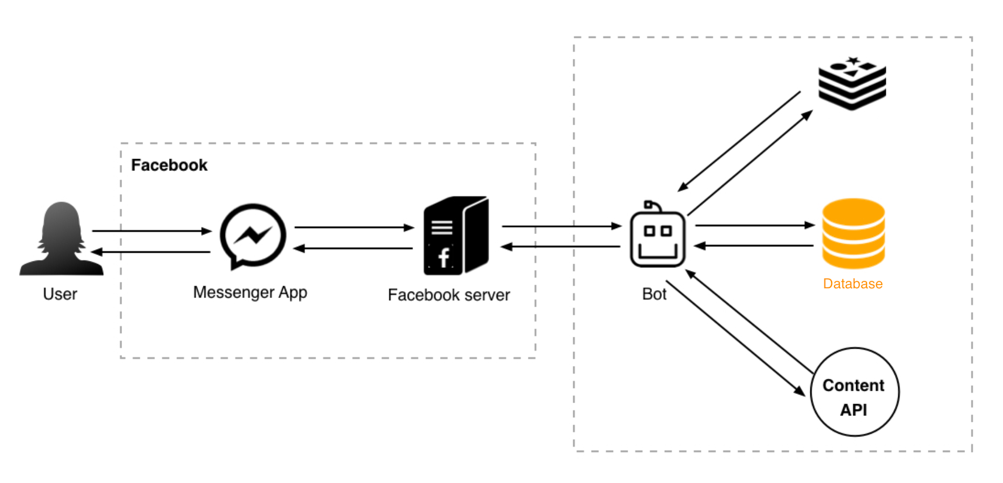
\includegraphics[width=\linewidth]{./pictures/facebook_overview}}
\caption{Overview of the system}
\label{fig:facebook_overview}
\end{figure}
\FloatBarrier

Using the Facebook Messenger as interface for our service, the user doesn't have to download a separate application and is already accustomed to navigate within the application and its usage. In order to use the service the user has to search for the \emph{Before Order} page on Facebook and send the profile a message by clicking the \emph{Send Message} button.

\begin{figure}[htbp]
\centerline{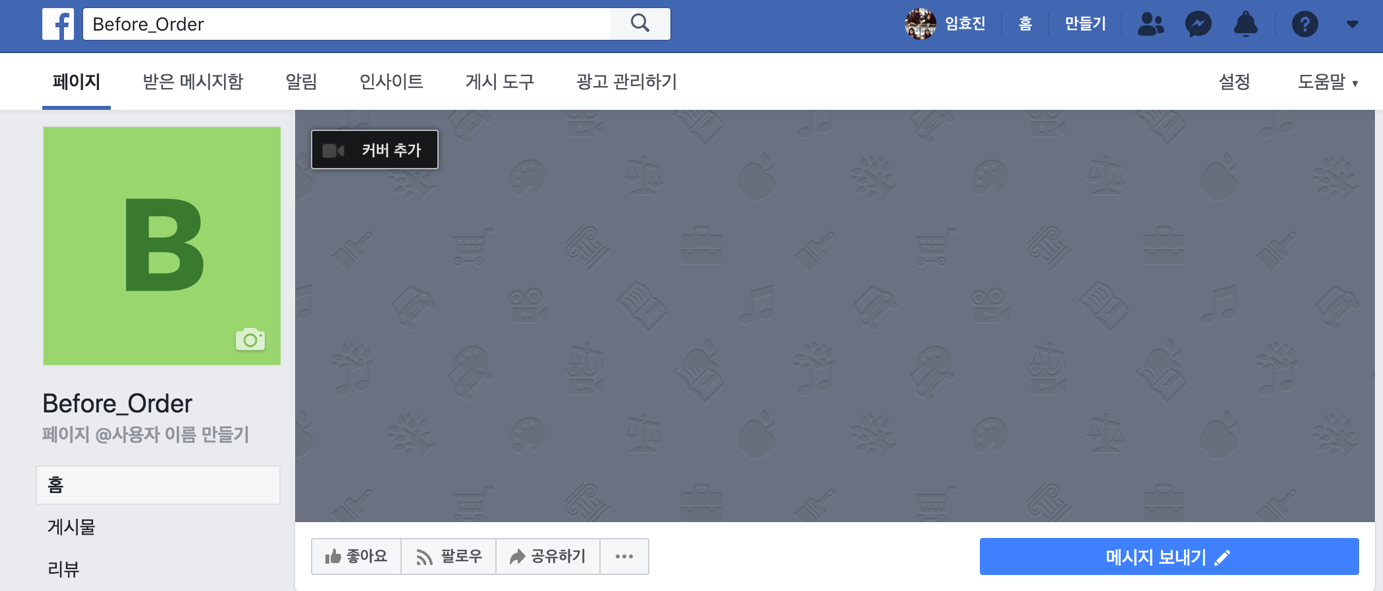
\includegraphics[width=\linewidth]{./pictures/facebook_profil}}
\caption{Chatbot profil on Facebook}
\label{fig:facebook_profil}
\end{figure}
\FloatBarrier

\subsubsection{Facebook messenger}

Given that the user has sent a message to the \emph{Before Order} service, the chat will be easily accessible from then on in the chatroom section of the Facebook Messenger application.

\begin{figure}[htbp]
\centerline{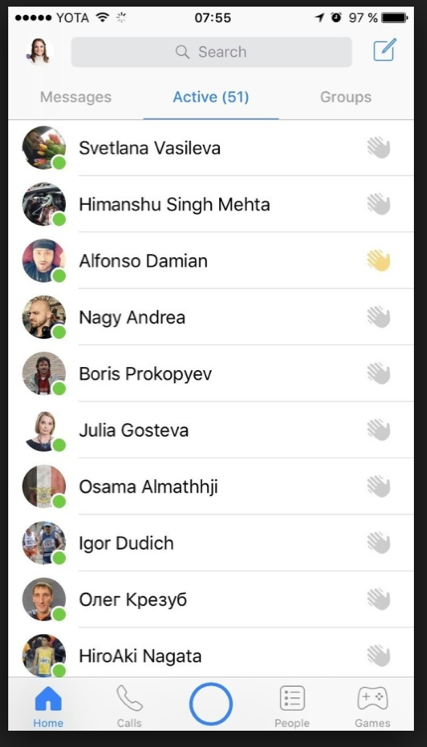
\includegraphics[height=\custompicheight]{./pictures/facebook_friends}}
\caption{Homescreen of the Facebook Messenger}
\label{fig:facebook_friends}
\end{figure}
\FloatBarrier

By selecting \emph{Before Order} from the list, the user is now able to provide a picture or dish names in the Korean alphabet to the chatbot by sending an image or a text message as shown in Fig. \ref{fig:facebook_message}

\begin{figure}[htbp]
\centerline{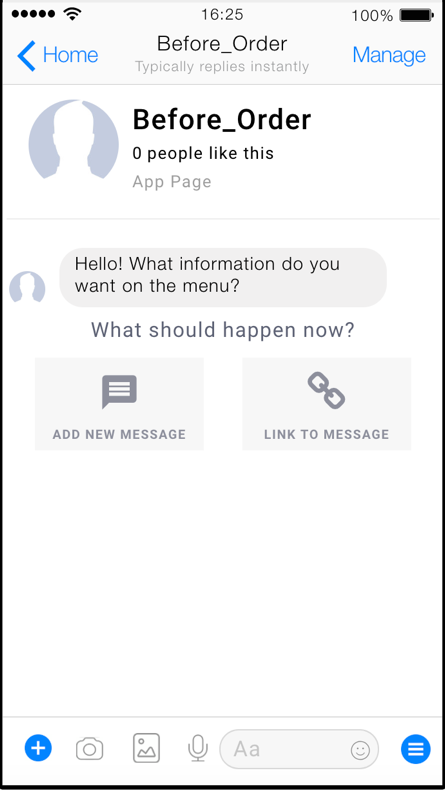
\includegraphics[height=\custompicheight]{./pictures/facebook_message}}
\caption{Chatroom with the \emph{Before Order} chatbot}
\label{fig:facebook_message}
\end{figure}
\FloatBarrier

\subsubsection{Chatbot input}

If the user sends the menu in form of a picture, the dish names have to be spelled out and need to be visible. The user can either send a picture that he took in the past or use the camera function in the Facebook Messenger to capture a picture and directly send it to the chatbot.

\begin{figure}[htbp]
\centerline{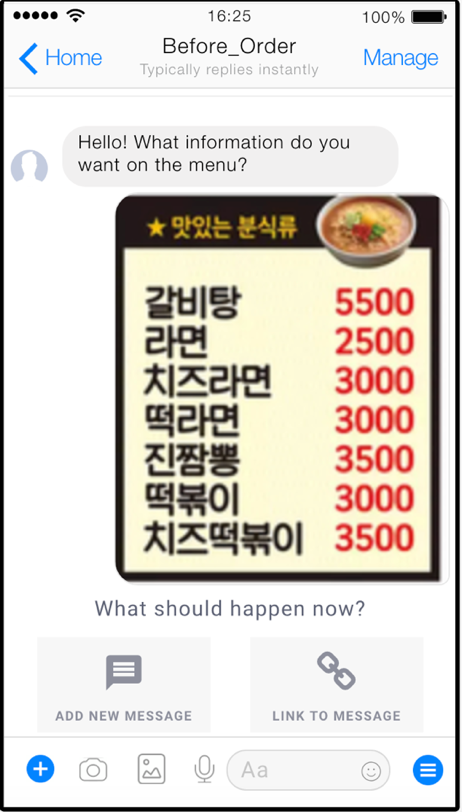
\includegraphics[height=\custompicheight]{./pictures/facebook_menu}}
\caption{Message to the chatbot including a picture of a menu}
\label{fig:facebook_menu}
\end{figure}
\FloatBarrier

Using a text recognition API and analyzing the image we are able to provide a list with all the found and supported dish names. The user is now able to select a dish that he wants more detailed information about as shown in Fig. \ref{fig:facebook_response}.

\begin{figure}[htbp]
\centerline{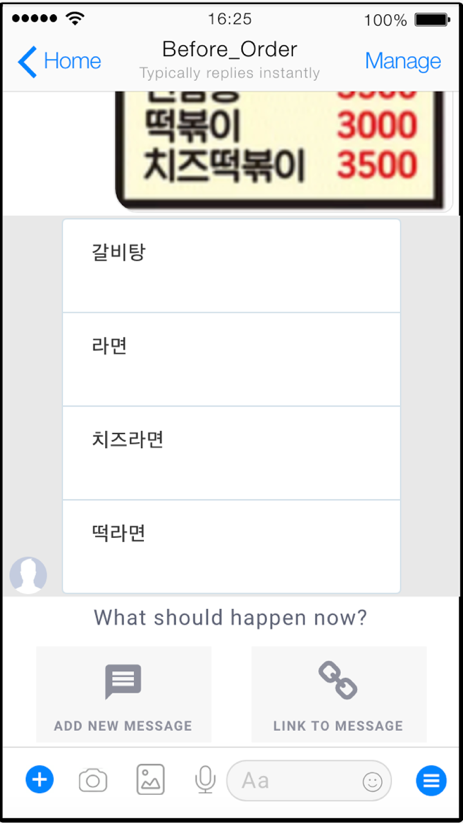
\includegraphics[height=\custompicheight]{./pictures/facebook_response}}
\caption{Response of the chatbot with all the found dishes}
\label{fig:facebook_response}
\end{figure}
\FloatBarrier

\begin{figure}[htbp]
\centerline{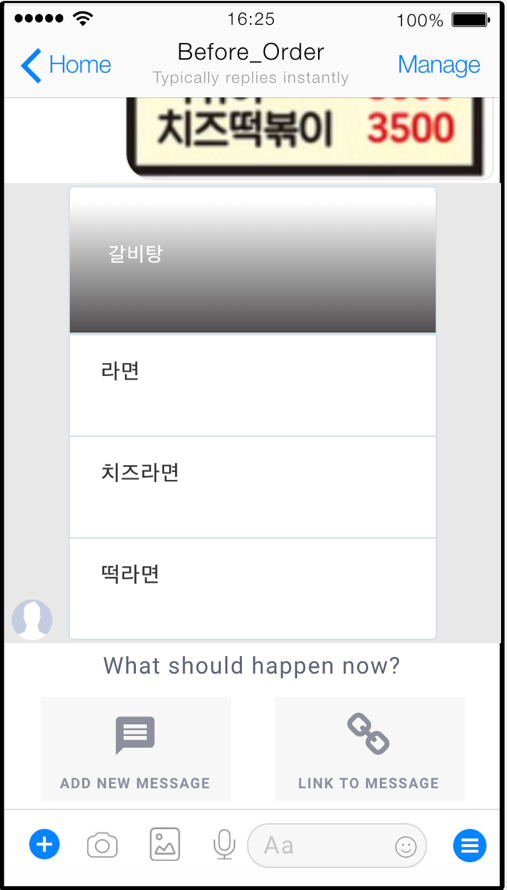
\includegraphics[height=\custompicheight]{./pictures/facebook_response_selection}}
\caption{User selecting a dish from the list}
\label{fig:facebook_response_selection}
\end{figure}
\FloatBarrier

\subsubsection{Processing of the input}

\begin{itemize}
\item Get the information from database

The information for dishes will be provided by our own database. Instead of using an open-source API for translating korean words to english we will be using an own mapping between english and korean dish names as the common translators don't support uncommon dish names or variants of dish names. Therefore each dish will have an english and an korean name associated with it to make it possible to search for dishes inside the database using korean letters. Hence most of the processes in and around the database will have to support and communicate using the UTF-8 encoding. The database will also contain a one or two sentence description for each dish, a list with its main ingredients and additional flags, such as \emph{spicy}. Managing and searching for information in this kind of database has the advantage, that:

    \begin{itemize}
    \item information for every dish is consistent and unlike as in popular search machines, such as \emph{Wikipedia} and \emph{Google}, every entry in the database will have the common information
    \item we can be sure information and names in the database refers to a dish, which enables us to filter out random textsequences and unrelated korean words and sentences
    \item we don't have to rely on the authenticity of information from a third party
    \end{itemize}

\item Server that can run chatbot and chatbot service

We will use Azure Virtual Server to run our chatbot. There are three parts in our chatbot service in the virtual machine. First one is a script that is connected with Facebook Chatbot API. This script will have scenario to answer users' requests and call other scripts to provide information to the users. Second one is to recognize the texts from the picture that users give using Computer Vision API, and the last one is for interacting with the database. When the chatbot gets the input from the users, it will call the script for text recognition. And the results will be sent again as a list format to the users. The other input that user chooses in the list will be given to the chatbot. Then chatbot will call the script for retrieving data from the database and return the detailed information about the dish to the user.

\item Vision api connection

When chatbot calls a program that is connected with Computer Vision API, It will send the picture to the Computer Vision API and get the results from it. It includes a request using the key and endpoint of the Computer Vision API. When the program sends the request to the API, it gets a result as a json format. The program also includes refine part. It refines the result text and make a result as a list format.  it returns the list-format result to the chatbot.
\end{itemize}
\FloatBarrier

\subsubsection{Chatbot output}

\begin{figure}[htbp]
\centerline{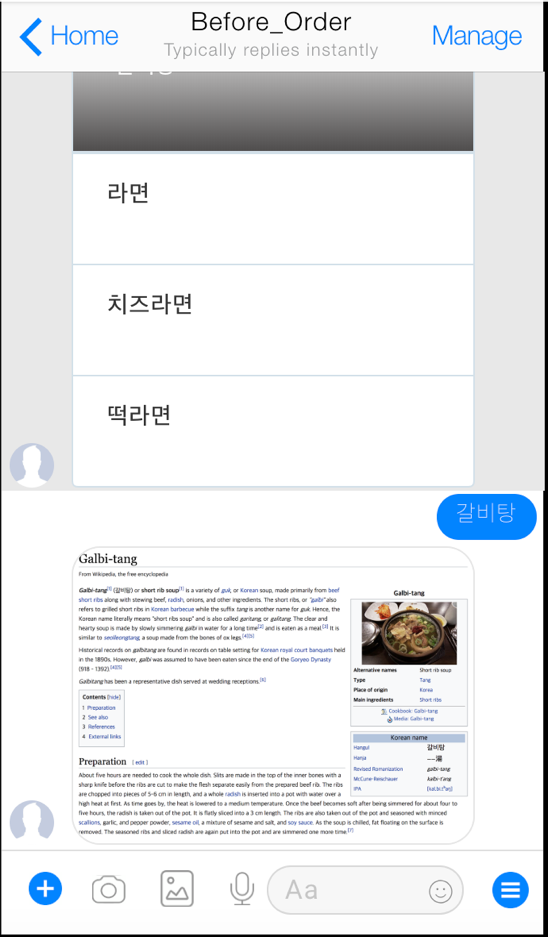
\includegraphics[height=\custompicheight]{./pictures/facebook_dish_information}}
\caption{Detailed informations about the selected dish}
\label{fig:facebook_dish_information}
\end{figure}
\FloatBarrier

Although we can not represent it in this prototype, we plan to provide information from our internal database. Users will be able to receive images of the dishes and a detailed description with ingredients.

\subsubsection{Exit}
If you need information about other menus, please feel free to send us a message.

\end{document}
